\chapter{Experimente}
\label{cha:experimente}

\section{Vereinfachte Kalibrierung}
\label{sec:vereinfachtekalib}

Eine andere M"oglichkeit, als in \ref{sec:kalibrierung} erl"autert, eine Kamera zu kalibrieren, ist mit Hilfe eines rechteckigen Kalibrierobjektes. In unserem Fall handelt es sich, wie in \ref{fig:klammern} zu sehen ist, um die Verpackung von Heftklammern.
 
\begin{figure}[H]
	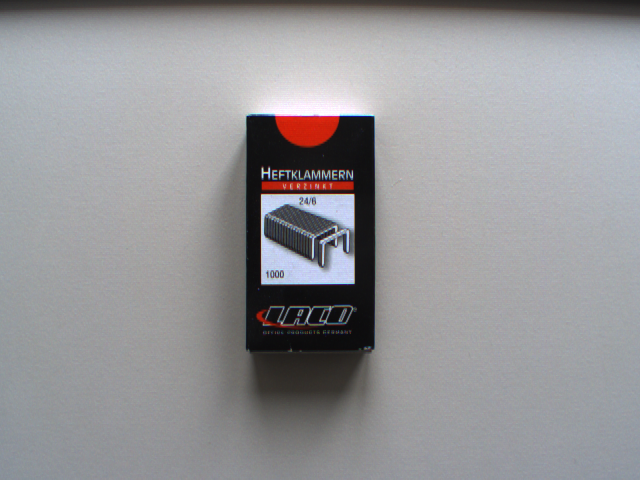
\includegraphics[scale=0.5]{bilder/experimentcalib}
	\caption[Kalibrierobjekt]{Kalibrierobjekt}
	\label{fig:klammern}
\end{figure}

\noindent Die Formel zur Berechnung der Brennweite $f_x$ und $f_y$ ergibt sich aus den Formeln \newline
$f_x=\frac{\Delta x'}{x}z$ und $f_y=\frac{\Delta y'}{y}z$\newline
bei $\Delta x$ und $\Delta y$ handelt es sich um die jeweiligen Seitenl"angen des Kalibrierobjekts.\newline
$\Delta x'$ und $\Delta y'$ sind die L"angen der Seiten des Kalibrierobjekts in Pixelwerten. $z$ ist der Abstand zwischen Linse und Objekt \cite{PCV} \cite{CVF}.

\begin{figure}[H]
	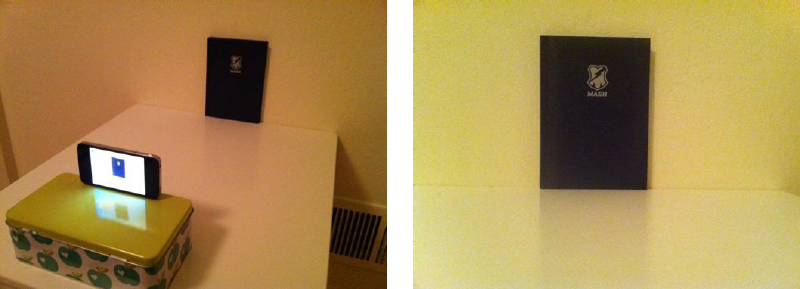
\includegraphics[scale=1.0]{bilder/simple_calib}
	\caption[Vereinfachte Kalibrierung]{Vereinfachte Kalibrierung}
	\small Quelle: Solem 2012
	\label{fig:simplecalib}%
\end{figure}

\noindent Wie in \ref{fig:simplecalib} zu sehen ist, muss das Kalibrierobjekt senkrecht auf eine plane Oberfl"ache gestellt werden. So auch die Kamera. Die Kamera muss dann so ausgerichtet werden, dass das Objekt im Bild genau zentriert und entlang der Bildzeilen und -spalten ausgerichtet ist \cite{CVF}.\newline
Obwohl diese Kalibrierung sehr ungenau erscheint, wurde ein dennoch relativ geringer Reprojection-Error, der den Wert ? hat, ermittelt. Der wie in \cite{cal} ermittelte Wert, von ? ,ist dennoch besser.

\section{Tiefeninformationen}
\label{sec:expiefeninformationen2}

Die Methode Tiefeninformationen zu ermitteln, wie es in \ref{sec:tiefeninformationen} erl"autert wird, wurde vorerst mit einem Experiment validiert.

\begin{figure}[!htb]
	\minipage{0.32\textwidth}
	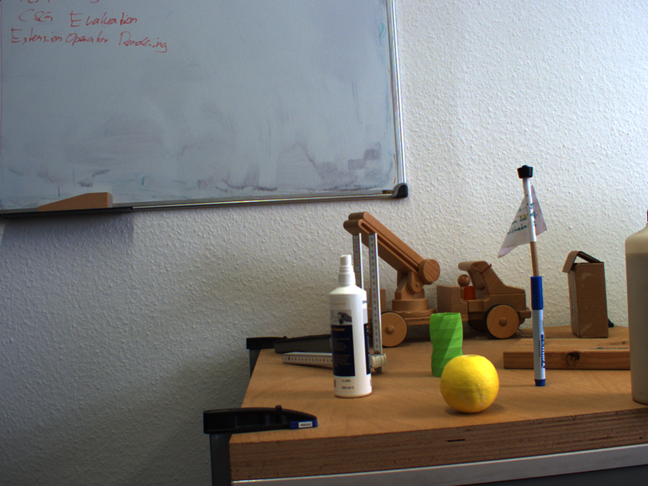
\includegraphics[width=\linewidth]{bilder/depth_left}
	\caption{Tiefe links}\label{fig:depthleft}
	\endminipage\hfill
	\minipage{0.32\textwidth}
	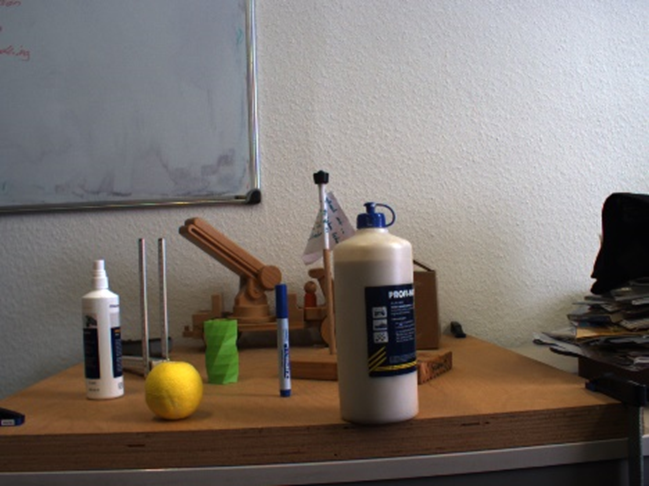
\includegraphics[width=\linewidth]{bilder/depth_right}
	\caption{Tiefe rechts}\label{fig:depthright}
	\endminipage\hfill
	\minipage{0.32\textwidth}%
	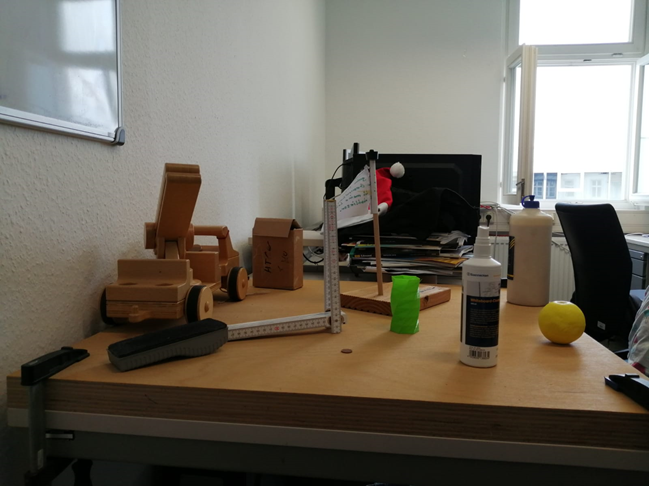
\includegraphics[width=\linewidth]{bilder/depth_side}
	\caption{Tiefe seitlich}\label{fig:depthside}
	\endminipage
\end{figure}

\noindent Mit dem Stereo-System wurden zwei Aufnahmen einer Szene aufgenommen (\ref{fig:depthleft} und \ref{fig:depthright}). Auf dem seitlichen Bild \ref{fig:depthside}, sieht man die tats"achliche Tiefe der Objekte im Bild.

\begin{figure}[!htb]
	\minipage{0.48\textwidth}
	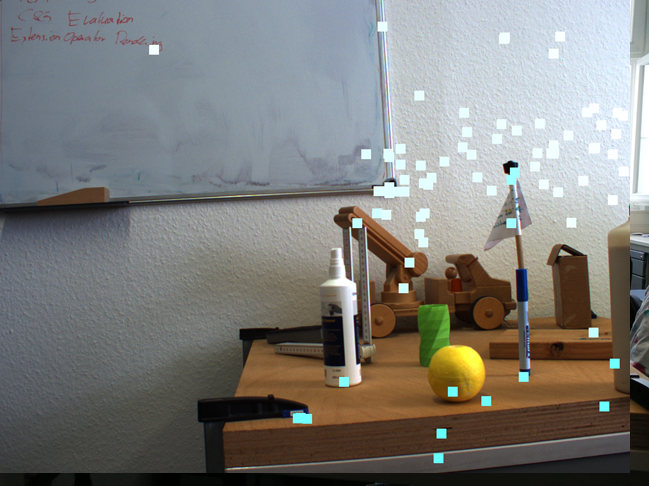
\includegraphics[width=\linewidth]{bilder/depth_result}
	\caption{Tiefeninformation Punkte}\label{fig:depthpoints}
	\endminipage\hfill
	\minipage{0.48\textwidth}
	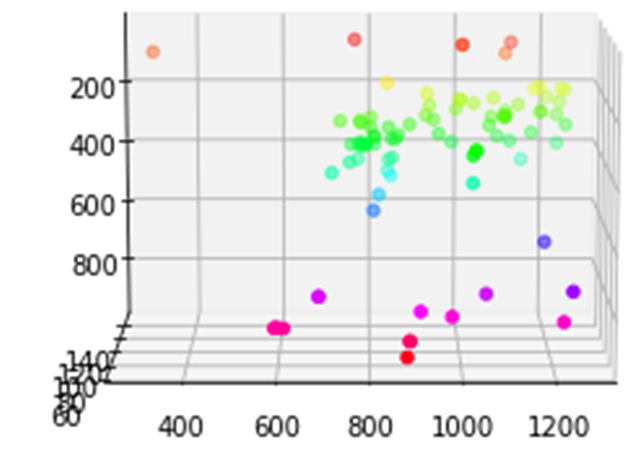
\includegraphics[width=\linewidth]{bilder/depth_coord}
	\caption{Tiefeninformation 3D-Plot}\label{fig:depthplot}
	\endminipage\hfill
\end{figure}

\noindent Auf den zwei Bildern der Szene wurden hier vorest h"andisch, dann mittels des SIFT-Algorithmus Referenzpunkte ermittelt, zu denen die Tiefe berechnet werden sollte. Der Abstand der beiden Kameras $B$ wurde hier h"andisch mit einem Lineal ausgemessen. Der Wert hier f"ur musste allerdings mehrere Male angepasst werden, da es wegen des Kamera-Geh"auses nicht klar war, wo genau sich der Sensor der Kamera befindet.\newline
Dann wurde die, wie in \ref{sec:tiefeninformationen} erw"ahnte Formel angewandt, um den Wert der $Z$-Achse der jeweiligen Punkte zu ermitteln.\newline
Mittels eines selbst geschriebenem Algorithmus, der Werte mit im Mittel großem $Z$ wei"slich und Werte mit im Mittel kleinem $Z$ hellblau einf"arbt, kann man sich die Informationen zur Tiefe auf einem Bild darstellen.\newline
In \ref{fig:depthpoints} kann man gut erkennen, dass Objekte, die n"aher an der Kamera stehen, mit einem hellen blau markiert sind. Objekte, die weiter entfernt sind, mit einem wei"slichem Farbton. Durch dieses Experiment war es uns m"oglich zu Validieren, dass unser Ansatz der Richtige war.